% !Mode\dots ``TeX:UTF-8''
% !TEX root = ../bare_jrnl.tex


\section{The online observability of \BCNs}
\label{sec:online}

%In this section we propose the online observability to solve the problem mentioned in {\em Section \ref{sec:pre}}, and we will introduce its related information in detail. 
%
%In the rest of this section, firstly we introduce the inspiration for the online observability. Secondly we define derivation function. Thirdly we present the definition of $k$-step determinability. Finally, we give the formal definition of the online observability of \BCNs\ by derivation function and $k$-step determinability, and compare it with four existing observability.

%\subsection{Inspiration}


%As we mentioned in {\em Section \ref{sec:pre}}, we can determine the initial states of \BCNs\ by the third existing observability. \tl{(2)why but here?} But i
%{\color{red} (2)}In the third observability, the $\mathsf{s}(0)$ of a \BCN\ can be determined iff there exists an finite input sequence $\mathsf{I}$ that determine $\mathsf{s}(0)$.

%But we foud that we can derive the set of possible initial states $\mathsf{S}(0)$ by initial output $\mathsf{o}(0)$ we observe
%\[\mathsf{S}(0)=\{\mathsf{s}(0)\in \Delta_N|\ h( \mathsf{s}(0))=\mathsf{o}(0)\}.\]
%\tl{(3)i do not see logical connection here}
%Then if for every $\mathsf{S}^{i}(0)=\{\mathsf{s}(0)\in \Delta_N|\ h( \mathsf{s}(0))=\mathsf{o}^{i}(0)\}$, there is an input sequence $\mathsf{I}^{i}\in(\Delta_M)^k$ for some $k>0$, such that for any distinct states $\mathsf{s}^{x}(0)$, $\mathsf{s}^{y}(0) \in \mathsf{S}^{i}(0)$ implies $(HF)^k_{\mathsf{s}^{x}(0)}(\mathsf{I^i})\neq (HF)^k_{\mathsf{s}^{y}(0)}(\mathsf{I^i})$, we can determine the initial $\mathsf{s}(0)$ too. In this case, the requirements for a \BCN\ to determine its initial state would be easier to meet. \tl{(4)this because is connected to the previous sentence?}Because the corresponding input sequences $\mathsf{I}^{i}$ of different sets of possible initial states $\mathsf{S}^{i}(0)$ can be different. While in the third existing observability the $\mathsf{I}^{i}$ has to be identical.

%Furthermore, we can derive the set of possible states $\mathsf{S}(1)$ by the outputs $\mathsf{o}(0)$ and $\mathsf{o}(1)$ we observe and the input $\mathsf{i}(0)$ 
%\[\mathsf{S}(1)=\{\mathsf{s}(1)|\mathsf{s}(0)\in \mathsf{S}(0),\ \mathsf{s}(1)=f({\mathsf{i}(0)},{\mathsf{s}(0)}),\ h(\mathsf{s}(1))=\mathsf{o}(1)\}.\]

%And if for every $\mathsf{S}^{i}(1)$ we derived, 
%\begin{itemize}
%  \item  there is an input sequence $\mathsf{I}^{i}\in(\Delta_M)^k$ for some $k>0$, such that for any distinct states $\mathsf{s}^{x}(1)$, $\mathsf{s}^{y}(1) \in \mathsf{S}^{i}(1)$ implies $(HF)^k_{\mathsf{s}^{x}(1)}(\mathsf{I^i})\neq (HF)^k_{\mathsf{s}^{y}(1)}(\mathsf{I^i})$;
%  \item  and for every $\mathsf{s}^{x}(1)$ $\in \mathsf{S}^{i}(1)$ there exists only one corresponding $\mathsf{s}^{x}(0)$ $\in \mathsf{S}^{i}(0)$ such that $\mathsf{s}^{x}(1)=f({\mathsf{i}(0)},{\mathsf{s}^{x}(0)})$,
%\end{itemize} 
%then we can determine the initial state too. And in this case, the requirements for the \BCN\ to determine the initial state would be further easier to meet. Because the corresponding input sequences $\mathsf{I}^{i}$ of different sets of possible states $\mathsf{S}^{i}(1)$ can be different. 

%\tl{(5)this therefore is repeating what was said before?}
%Therefore, we have that if we utilize sets of possible states we derived more, it would be easier for a \BCN\ to meet the requirements to determine its initial state. According to this rule, we propose the online observability. 
%\tl{(6)does this mean that online observability is dependent on a particular rule?}
 %by taking the determining procedure once, we only need to complete the following procedure.
 %To improve the weakness of the algorithm corresponding to {\bf Type-III} observability, we propose a new algorithm (mentioned in {\em Section \ref{sec:intro}}) to determine $\mathsf{s}(0)$. Based on this new algorithm, we propose the online observability, viz., a \BCN\ is online observable if its $\mathsf{s}(0)$ can be determined by this new algorithm. %And we call the {\bf Type-III} observability offline observability.

%And in this procedure, instead of finding the  $\mathsf{I}$ to determine $\mathsf{s}(0)$ before we take the determining procedure. We use the $\mathsf{S}(t)$ we derive at every time step $t$ to adaptively construct $\mathsf{I}$. 

  %\tl{do you mean that the procedure terminates?} \gs{Yes} 


%We will formally define it in following subsections, 
%%\tl{(7)this implies that online is at least as powerful as offline, but why it is stronger?}
%%Such that the requirements to determine the \BCNs' initial state would be easiest to meet. Thus, a \BCN\ satisfies the online observability iff its initial state $\mathsf{s}(0)$ can be determined for every $\mathsf{s}(0) \in \Delta_N$. 
%its formal definition should define  
%%After introducing the idea of the online observability, we briefly present how to determine the initial state of a \BCN. 
%\begin{itemize}
%\item the way to derive $\mathsf{S}(t)$ by $\mathsf{o}(t)$, $\mathsf{i}(t-1)$ and $\mathsf{S}(t-1)$ should be described, %So we define the derivation function to solve this problem.
%\item  and the way to derive $\mathsf{i}(t)$ by $\mathsf{S}(t)$ to guarantee that $\mathsf{s}(0)$ can be determined. %Thus we define the $k$-step determinability for $\mathsf{S}(t)$ which means that we can determine $\mathsf{s}(t)$ by $\mathsf{S}(t)$ in $k$ time steps.
%\end{itemize} 


%Therefore, we have the definition of the online observability that a \BCN\ is online observable if for every $\mathsf{S}^{i}(0)$ we derived, there exists a $k^i\ge 0$ such that the $\mathsf{S}^{i}(0)$ is $k^i$-step determinable.

%\tl{(8)this means that the "definition" is dependent on a particular way to define $S(t)$ and $i(t)$. In other words, if one gives a different way to define $S(t)$ and $i(t)$, you would have another definition of online observability. This suggests that the def of online observability is not robust.}


%-------------------------------------
%-------------------------------------
To formally define the online observability, we start with the derivation function $\Ded( \mathsf{S},  \mathsf{i},  \mathsf{o})$ which formalize how to determine the set $\mathsf{S}(t)$ of possible valuations of $\mathsf{s}(t)$ of a \BCN\ by its updating rules.  %The definition of it is as follows.

Firstly, we write 

\begin{equation*}
\begin{split}
\xi :  (\mathcal{I}\cup\varepsilon) \times\mathcal{S} \mapsto\mathcal{S},\ \xi (\mathsf{i}, \mathsf{s})= \left\{
\begin{array}{rcl}
\sigma( \mathsf{i}, \mathsf{s})      &      & {\mathsf{i}\neq \varepsilon}\\
\mathsf{s}       &      & {\mathsf{i}= \varepsilon}
\end{array} \right. 
\end{split}
\end{equation*}
where $\varepsilon$ presents empty input.
%\begin{definition}[$\Ded( \mathsf{S},  \mathsf{i},  \mathsf{o})$] 
%$2^{\Delta_N}$ be the power set of states; \tl{in a def, please do not introduce notations}
%$(\Delta_M\cup\varepsilon)$ be the set of inputs and $\varepsilon$ means empty input; 
%$(\Delta_Q\cup\varepsilon)$ be the set outputs and $\varepsilon$ means empty output.
%If $\mathsf{o}\neq \varepsilon$
%\begin{equation*}
% \Ded( \mathsf{S},  \mathsf{i},  \mathsf{o})=\{  \xi(\mathsf{i}, \mathsf{s} ) \mid  \mathsf{s} \in \mathsf{S},  \rho(\xi(\mathsf{i}, \mathsf{s} ))=\mathsf{o}\}
%\end{equation*}
%If $\mathsf{o}= \varepsilon$
%\begin{equation*}
%\Ded( \mathsf{S},  \mathsf{i},  \mathsf{o})=\{  \xi(\mathsf{i}, \mathsf{s} ) \mid  \mathsf{s} \in \mathsf{S}\}
%\end{equation*}

Then the $\Ded( \mathsf{S},  \mathsf{i},  \mathsf{o})$ is defined as follows.
\begin{equation}
\begin{split}
\Ded&:2^{\mathcal{S}_\BB}\times(\mathcal{I}\cup\varepsilon)\times(\mathcal{O}\cup\varepsilon)\mapsto2^{\mathcal{S}_\BB},\\
\Ded( \mathsf{S},  \mathsf{i},  \mathsf{o})&= \left\{
\begin{array}{rcl}
\{  \xi(\mathsf{i}, \mathsf{s} ) \mid  \mathsf{s} \in \mathsf{S},  \rho(\xi(\mathsf{i}, \mathsf{s} ))=\mathsf{o}\}     &      & {\mathsf{o}\neq \varepsilon}\\
\{  \xi(\mathsf{i}, \mathsf{s} ) \mid  \mathsf{s} \in \mathsf{S}\}       &      & {\mathsf{o}= \varepsilon}
\end{array} \right. 
\end{split}
\end{equation}
%\begin{equation*}
%\begin{split}
%&\Ded( \mathsf{S},  \mathsf{i},  \mathsf{o})=\{  \mathsf{s}'\in\Delta_N|\\
%& \mathsf{s}'=  \mathsf{s} \in \mathsf{S}, \ h(\mathsf{s}')=\mathsf{o}\ if\ \mathsf{o}\neq \varepsilon\},
%\end{split}
%\end{equation*}
where  $\varepsilon$ presents empty input or empty output.
%\tl{check whether this is what you want!?}\gs{It is ok.}
%\end{definition}$\mathsf{S}\in 2^{\mathcal{S}_\BB}$, $\mathsf{i} \in (\mathcal{I}\cup\varepsilon)$, $\mathsf{o} \in (\mathcal{O}\cup\varepsilon)$, and

 And then, the set $\mathsf{S}(t)$ of possible valuations of $\mathsf{s}(t)$ of a \BCN\ $\BB$ is defined as follows. 
 \begin{definition}[$\mathsf{S}(t)$] Given $\mathsf{I}[k]=\mathsf{i}(0)\ldots\mathsf{i}(k-1)$, $\mathsf{o}(0)$ and $\mathsf{O}[k]=(HF)^k_{\mathsf{s}(0)}(\mathsf{I}[k])=\mathsf{o}(1)\ldots\mathsf{o}(k)$, %for every $t\le k$, 
	\[\mathsf{S}(t)=\left\{
\begin{array}{rcl}
\Ded\left(\mathcal{S}_\BB,\varepsilon,\mathsf{o}(0)\right)      &      & {t=0}\\
\Ded\left(\mathsf{S}(t-1),\mathsf{i}(t-1),\mathsf{o}(t)\right)       &      & 0<t\leq k
\end{array} \right. .\]

\end{definition}
\begin{example}
In the \BCN\ mentioned in {\em Example \ref{exa:2}}, if $\mathsf{o}(0)=\delta_4^0$, then \[\mathsf{S}(0)=\Ded\left(\mathcal{S}_\BB,\varepsilon,\delta_4^0\right)=\{\delta_{16}^0,\delta_{16}^1,\delta_{16}^2\}.\]
%If the possible states set $\mathsf{S}=\{\delta_{16}^0$, $\delta_{16}^1$, $\delta_{16}^2\}$ and we input $\delta_4^0$ observe $\delta_4^2$, then we can derive that the set of possible new states can be $\delta_{16}^{9}$ or  $\delta_{16}^{10}$.
 \label{exa:8}
 \end{example}   
 

 
 
%\subsection{$K$-step determinability}
%{\color{red} (10)} We propose the 

As the next step, we introduce a predicate $\Ks(\mathsf{S}(t))$ for $\mathsf{S}(t)$ to depict that we can determine the $\mathsf{s}(t)$ at time $(t+\Ks(\mathsf{S}(t))$ for every $\mathsf{s}(t)\in \mathsf{S}(t)$. 
 %\tl{(10)$k$-step determinability is a predicate, can you write in this form?}
\begin{definition}[$\Ks(\mathsf{S})$] 
For a non-empty set $\mathsf{S}\subseteq\mathcal{S}_\BB$
 \begin{itemize}
 \item   if $|\mathsf{S}|=1$ then $\Ks(\mathsf{S}$)=0;
 \item  if $|\mathsf{S}|>1$ and there is an input $\mathsf{i} \in \mathcal{I}$ such that % $\Ks(\mathsf{S})=\min(\{\max\{\Ks(\Ded(\mathsf{S},\mathsf{i}^{x},\mathsf{o}^{j}))| \Ded(\mathsf{S},\mathsf{i}^{x},\mathsf{o}^{j})\ne \emptyset, \mathsf{o}^{j}\in\Delta_Q\}||\Ded(\mathsf{S},\mathsf{i}^{x},\varepsilon)|=|\mathsf{S}|, \mathsf{i}^{x} \in \Delta_M\})+1$ 
 \begin{itemize}
 \item  $|\Ded(\mathsf{S},\mathsf{i},\varepsilon)|=|\mathsf{S}|$, and 
 \item   for every $\mathsf{o} \in \mathcal{O}$, $\Ded(\mathsf{S},\mathsf{i},\mathsf{o})\ne \emptyset$ implies $\Ks(\Ded(\mathsf{S},\mathsf{i},\mathsf{o}))< k$;
 \end{itemize} 
 and there is not any $\mathsf{i}' \in \mathcal{I}$ which satisfies that
  \begin{itemize}
 \item  $|\Ded(\mathsf{S},\mathsf{i}',\varepsilon)|=|\mathsf{S}|$, and 
 \item   for every $\mathsf{o} \in \mathcal{O}$, $\Ded(\mathsf{S},\mathsf{i}',\mathsf{o})\ne\emptyset$ implies $\Ks(\Ded(\mathsf{S},\mathsf{i'},\mathsf{o}))< k-1$, 
 \end{itemize} 
then $0<\Ks(\mathsf{S})=k\ne \infty$.%, and we can input $\mathsf{i}^{i}$ to determine makes $\mathsf{S}$ $k$-step determinable.
 \item Otherwise, $\Ks(\mathsf{S})=\infty$.
 \end{itemize}
\end{definition}

%Then, in order to better illustrate this definition, we give the following example.
\begin{example}\label{exa:9}
As mentioned in the {\em Example \ref{exa:8}}, $|\mathsf{S}(0)|=3$, and there exists $\delta_{4}^3$ such that 
 \begin{itemize}
 \item  $|\Ded\left(\mathsf{S}(0),\delta_{4}^3,\varepsilon\right)|=|\{\delta_{16}^0,\delta_{16}^{13},\delta_{16}^6\}|$,
 \item   and for each $\mathsf{o}\in \mathcal{O}$
  \begin{itemize}
  \item   $\Ks(\Ded\left(\mathsf{S}(0),\delta_{4}^3,\delta_{4}^0\right))=\Ks(\{\delta_{16}^0\})=0$;
 \item  $\Ks(\Ded\left(\mathsf{S}(0),\delta_{4}^3,\delta_{4}^3\right))=\Ks(\{\delta_{16}^{13}\})=0$;
  \item  $\Ks(\Ded\left(\mathsf{S}(0),\delta_{4}^3,\delta_{4}^1\right))=\Ks(\{\delta_{16}^{6}\})=0$.
 \end{itemize}
 \end{itemize}
Thus $\Ks(\mathsf{S}(0))=1$, that is $\mathsf{s}(0)$ can be determined at time $1$ for every $\mathsf{s}(0)\in \mathsf{S}(0)$. 
\end{example}  

We propose a lemma for $\Ks(\mathsf{S})$.

\begin{lemma}
For the non-empty $\mathsf{S}^{1}$ and $\mathsf{S}^{2}$, if $\mathsf{S}^{1}\subseteq\mathsf{S}^{2}$ and $\Ks(\mathsf{S}^{2})\ne\infty$, then $\Ks(\mathsf{S}^{1})\le\Ks(\mathsf{S}^{2})$.%and $\mathsf{S}^{1}\subseteq \mathsf{S}^{2}$, 
  \label{lemm:1}
\end{lemma}

%Because of the length of the article, we put all the proofs in the {\bf Appendix}. With the {\em Lemma \ref{lemm:1}}, it is easy to propose the {\em Lemma \ref{lemm:2}}
%\begin{lemma}
%For the non-empty $\mathsf{S}^{1}$ and $\mathsf{S}^{2}$, if $\mathsf{S}^{1}\subseteq\mathsf{S}^{2}$ and $\Ks(\mathsf{S}^{2})\ne\infty$ then $\Ks(\mathsf{S}^{1})\ne\infty$.
%For the sets of possible states $\mathsf{S}^{1}$ and $\mathsf{S}^{2}$, if there exists a $k^{i}\ge 0$ such that $\mathsf{S}^{2}$ is $k^{i}$-step determinable, and $\mathsf{S}^{1}\subseteq \mathsf{S}^{2}$, then there exists a $k^{j}\ge 0$ that $\mathsf{S}^{1}$ is $k^{j}$-step determinable.
%\label{lemm:2}
%\end{lemma}
All the proofs in the {\bf Appendix~A~Proof}. 

We propose $\Ri(\mathsf{S}(t))$ for $\mathsf{S}(t)$ to depict that we can choose $\mathsf{i}(t)$ from $\Ri(\mathsf{S}(t))$ to determine $\mathsf{s}(t)$.

%\begin{definition}[$\Ri(\mathsf{S})$] 
\begin{equation*}
\begin{split}
\Ri&:2^{\mathcal{S}_\BB} \mapsto2^{\mathcal{I}},\\
\Ri(\mathsf{S})&=\{\mathsf{i}\in \mathcal{I}|\  |\Ded\left(\mathsf{S},\mathsf{i},\varepsilon\right)|=|\mathsf{S}|, \\
&\forall \mathsf{o} \in \mathcal{O}, \Ded(\mathsf{S},\mathsf{i},\mathsf{o})\ne \emptyset \rightarrow \Ks(\Ded(\mathsf{S},\mathsf{i},\mathsf{o}))\ne \infty\}
\end{split}
\end{equation*}
%\end{definition}
\begin{lemma}
For the non-empty $\mathsf{S}^{1}$ and $\mathsf{S}^{2}$, if $\mathsf{S}^{1}\subseteq\mathsf{S}^{2}$ and $\Ks(\mathsf{S}^{2})\ne\infty$, then $\Ri(\mathsf{S}^2)\subseteq\Ri(\mathsf{S}^1)$.
\label{lemm:2}
\end{lemma}

In {\em Section \ref{sec:deter}}, we will design the determinnation algorithm for the online observability based on {\em Lemma \ref{lemm:1}, \ref{lemm:2}}.
%, and we will represent the details in .
%==========================================================================================

%\subsection{Online observability}
%The online observability is formall defined as follows.

Then, the online observability can be defined.
\begin{definition}[Online Observability of  BCNs]
%\tl{(12)why $\epsilon$ is in the def? for which purpose?}
 A \BCN\ is observable
if for every $\mathsf{o}(0)\in  \mathcal{O}$, $\Ded(\mathcal{S}_\BB,\varepsilon, \mathsf{o}(0))\ne\emptyset$ implies $\Ks(\Ded\left(\mathcal{S}_\BB,\varepsilon,\mathsf{o}(0)\right))\ne\infty$.
\end{definition}

%In order to better illustrate the definition of online observability, we give the following example.

\begin{example}
In the \BCN\ mentioned in {\em Example \ref{exa:2}}.  
 \begin{itemize}
 \item $\Ks(\Ded\left(\mathcal{S}_\BB,\varepsilon, \delta_{4}^0\right))=1\ne \infty$;
 \item $\Ks(\Ded\left(\mathcal{S}_\BB,\varepsilon, \delta_{4}^1\right))=1\ne \infty$;
 \item $\Ks(\Ded\left(\mathcal{S}_\BB,\varepsilon, \delta_{4}^2\right))=2\ne \infty$;
 \item $\Ks(\Ded\left(\mathcal{S}_\BB,\varepsilon, \delta_{4}^3\right))=2\ne \infty$.
 \end{itemize}
 
Therefore this \BCN\ satisfies the online observability.%, thus we can determine the initial state of it even if its initial state can not be reset. And this \BCN\ is controllable, thus it is identifiable.  %Thus with the online observability we can research the \BCNs\ better.
\label{exa:10}



%its \State$(0)$ can be determined by this new algorithm for every \State$(0)$. Its formal definition will be presented in Section~\ref{sec:online}.  

We call this observability online observability, because we choose every $\mathsf{i}(t)$ to determine initial state $\mathsf{s}(0)$ based on the information of the inputs and outputs of \BCN\ we have collected so far at every time $t$, i.e. $\mathsf{i}(t)\in\Ri(\mathsf{S}(t))$. 

In contrast, in the {\bf type-III} observability, we determine the initial state $\mathsf{s}(0)$ of a \BCN\ by its recorded $\mathsf{O}[k]=\mathsf{o}(0)\ldots\mathsf{o}(k)$ after we input $\mathsf{I}[k]=\mathsf{i}(0)\ldots\mathsf{i}(k-1)$, and  we do not interfere with \BCN\ except for the logging of its inputs and outputs, thus we call it offline observability.


\end{example}  

\begin{lemma}
The {\bf Type-III} observability implies the online observability.
\label{lemm:4}
\end{lemma}

\begin{lemma}
The online observability implies the  {\bf Type-I} observability.
\label{lemm:3}
\end{lemma}

%With the existing first observability, we can distinguish every $\mathsf{s}^{i}(0)$ from other types of initial state, and we can also do this by the online obervability. Thus the online obervability implies the existing first observability. 



From the {\em Lemma \ref{lemm:3}}, {\em Lemma \ref{lemm:4}} and the implication relations between the existing four types of observability, we have the relations among all five types of observability shown in Fig.~\ref{fig:7}.
%In the existing third observability, we can determine the initial state $\mathsf{s}^{i}(0)$ of \BCN\ too. Thus the existing third observability implies the online obervability.

\begin{figure}[thpb]
      \centering
      \framebox{\parbox{3in}{\centerline{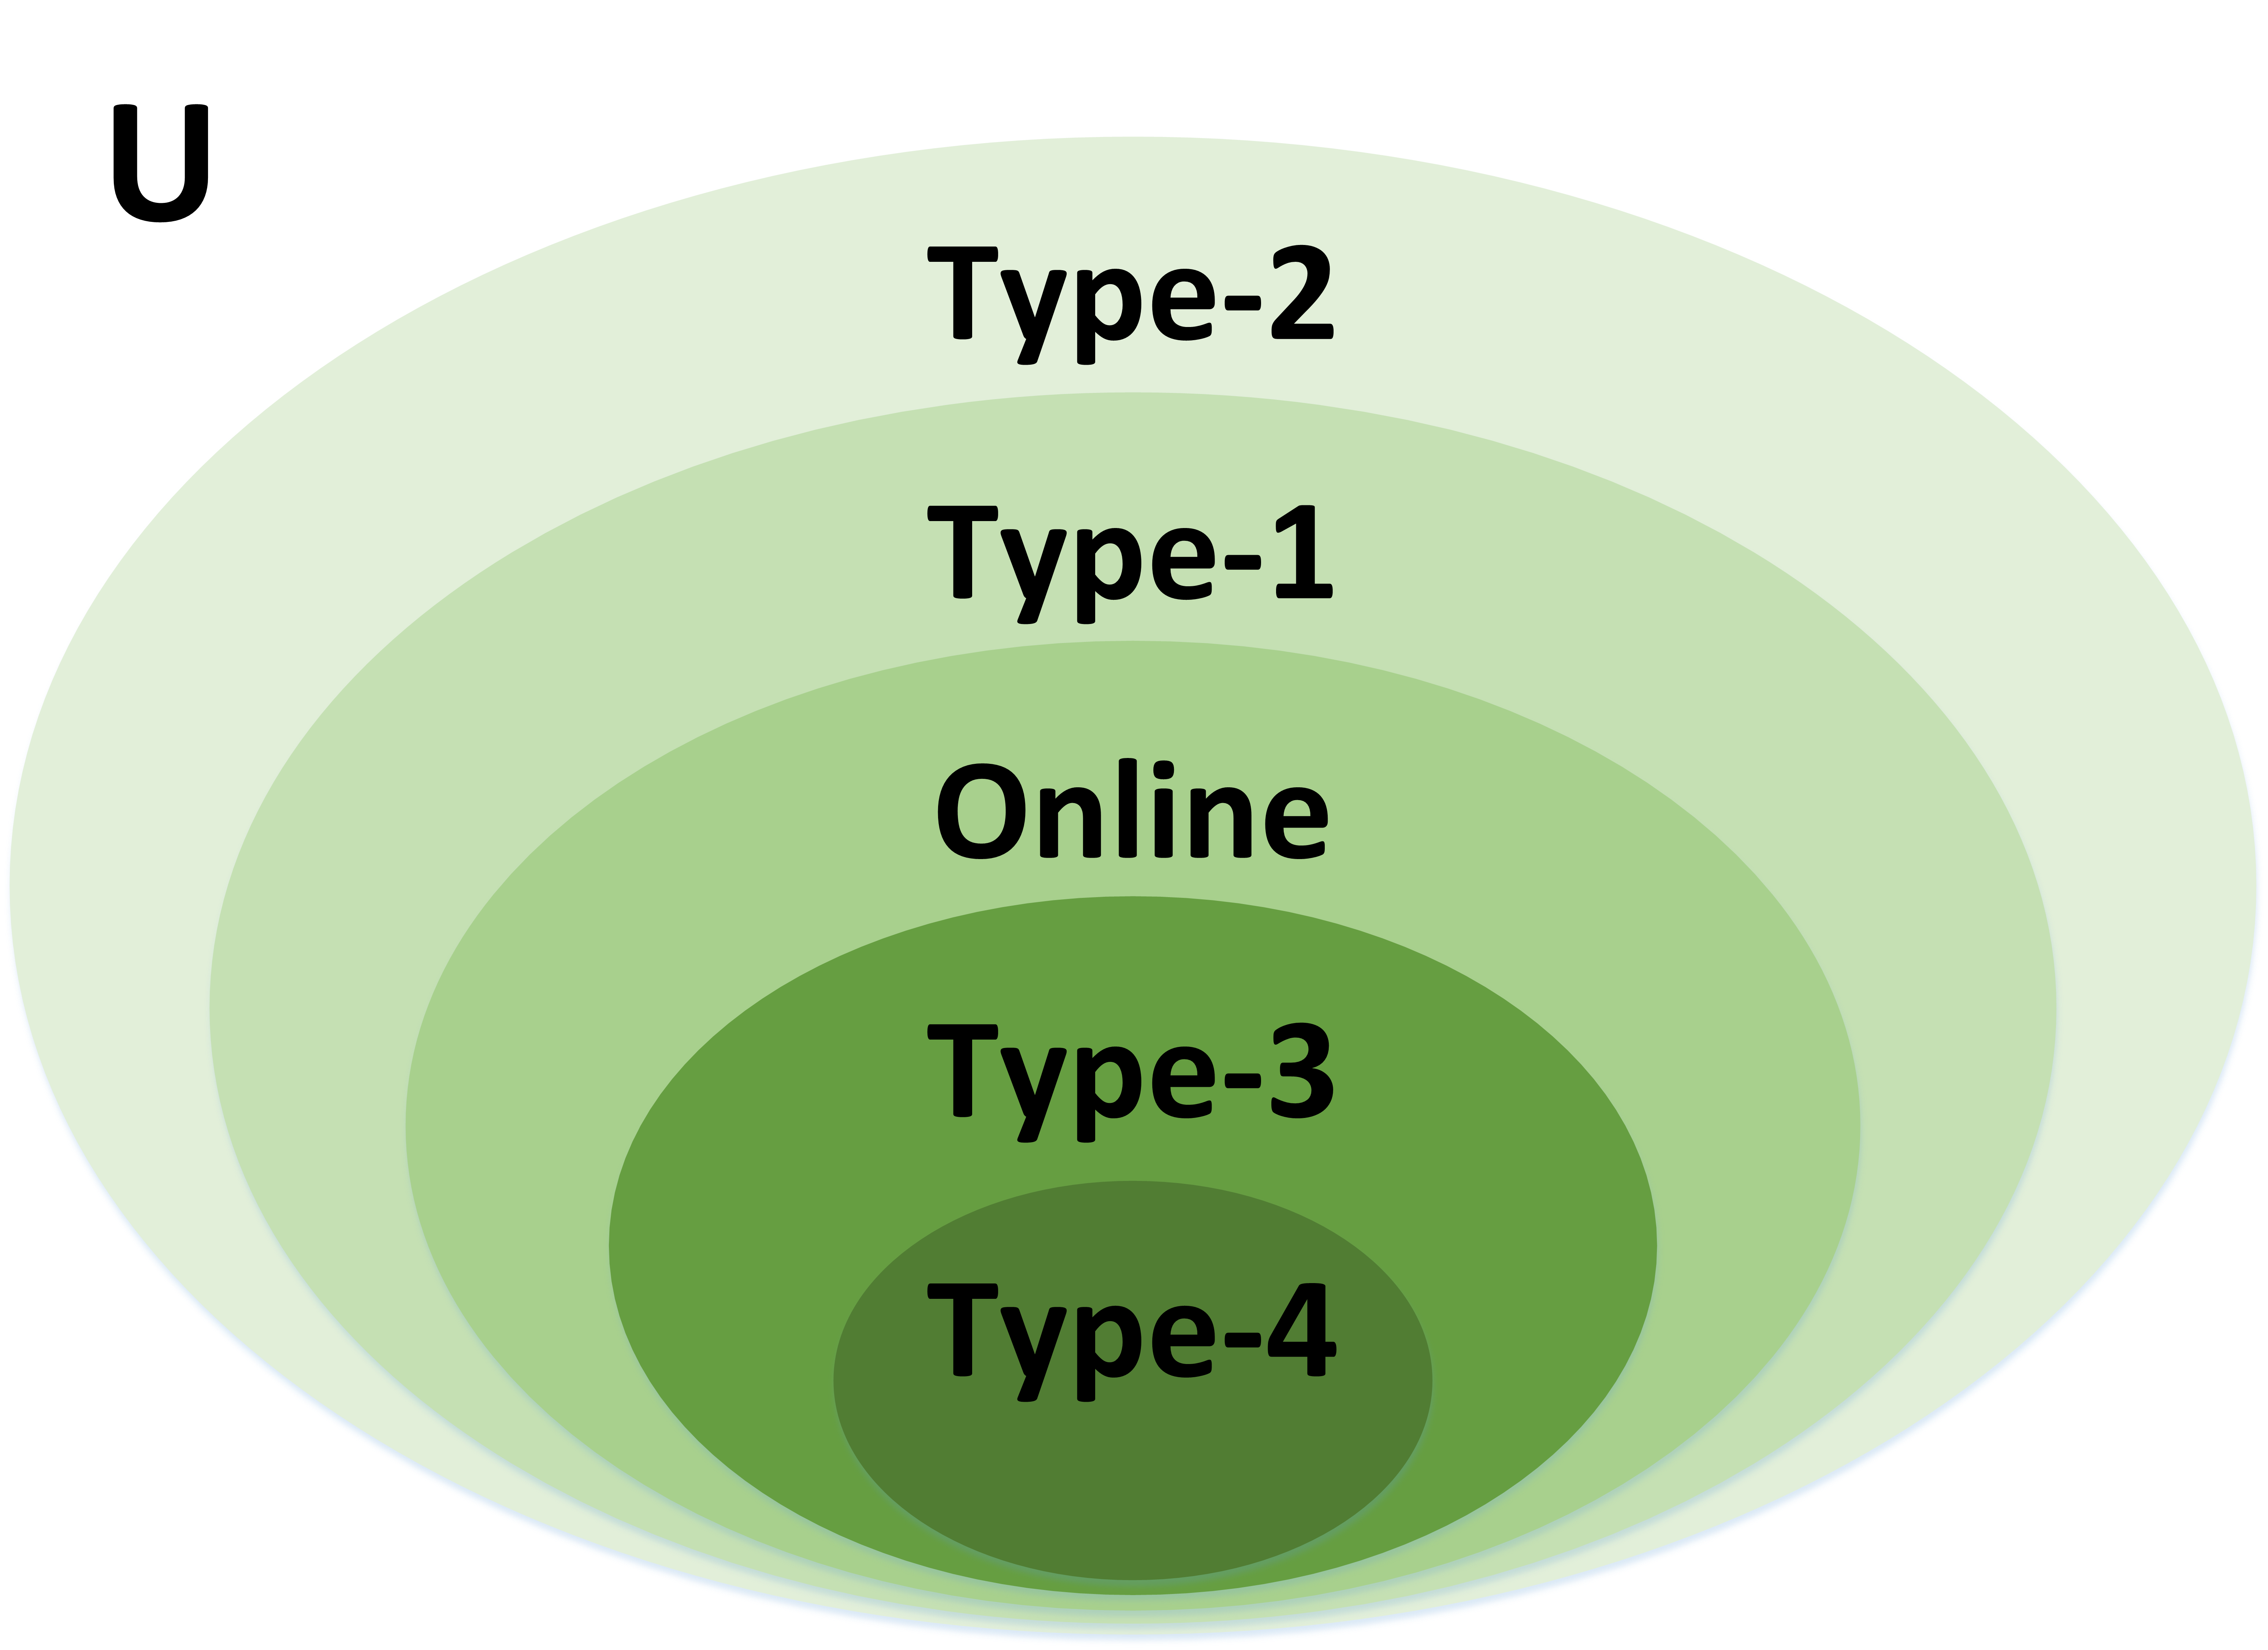
\includegraphics[scale=0.29]{figures/Fig11.png}} }} 
     \caption{The relationships graph between all five observability, where the area labelled with a type of observability presents the set of \BCNs\ which satisfy this type of observability, and  ``U" means all of the \BCNs.}
      \label{fig:7}
   \end{figure}

In conclusion, the online observability is the necessary and sufficient condition of determining the initial state $\mathsf{s}(0)$ of a \BCN\  without  resetting, %Because at every time $t$, we observe $\mathsf{o}(t)$ of \BCN\ and choose $\mathsf{i}(t)$ based on the information we have collected so far. 
and the identifiiability requires this condition. Thus, we can research the identification problem by the online observability instead of the {\bf Type-III} observability. 
%\subsection{Determining the intial state}




%\tl{(13)maybe you have done this, but I feel that one needs to highlight the advantages of this def. It is neither the strongest nor the weakest, why one should choose this?}

